
\documentclass[a4paper,11pt,fleqn]{article}
\usepackage{amsfonts}
\usepackage{amsthm}
\usepackage{graphicx}
\usepackage{fancyhdr}

\pagestyle{fancy}
% with this we ensure that the chapter and section
% headings are in lowercase.
%\renewcommand{\chaptermark}[1]{\markboth{#1}{}}
\renewcommand{\sectionmark}[1]{\markright{\thesection\ #1}}
\fancyhf{} % delete current setting for header and footer
\fancyhead[LE,RO]{\bfseries\thepage}
\fancyhead[LO]{\bfseries\rightmark}
\fancyhead[RE]{\bfseries\leftmark}
\renewcommand{\headrulewidth}{0.5pt}
\renewcommand{\footrulewidth}{0pt}
\addtolength{\headheight}{0.5pt} % make space for the rule
\fancypagestyle{plain}{%
\fancyhead{} % get rid of headers on plain pages
\renewcommand{\headrulewidth}{0pt} % and the line
}





\setlength{\parindent}{3em} \setlength{\oddsidemargin}{0in}
\setlength{\textwidth}{6.5in} % sets 1in left and right margins
\setlength{\topmargin}{0.0in} % change to 0.2in for regular latex
%\setlength{\headheight}{0in}
%\setlength{\footheight}{0.5in}
\setlength{\footskip}{0.5in}
\setlength{\textheight}{9.0in} %sets 1in top and bottom margins
%\renewcommand{\baselinestretch}{1} %set to 1.5 for double spacing.


\newtheorem{Prop}{Proposition}
\newtheorem{lemma}{Lemma}

\newcommand{\br}{{\mathbf r}}
\newcommand{\bA}{{\mathbf A}}
\newcommand{\ba}{{\bf a}}
\newcommand{\bb}{{\bf b}}
\newcommand{\bc}{{\bf c}}
\newcommand{\bC}{{\bf C}}
\newcommand{\bg}{{\bf g}}
\newcommand{\bG}{{\bf G}}
\newcommand{\bd}{{\bf d}}
\newcommand{\be}{{\bf e}}
\newcommand{\bs}{{\bf s}}
\newcommand{\bm}{{\bf m}}
\newcommand{\bn}{{\bf n}}
\newcommand{\bu}{{\bf u}}
\newcommand{\bv}{{\bf v}}
\newcommand{\bw}{{\bf w}}
\newcommand{\bx}{{\bf x}}
\newcommand{\bbf}{{\bf f}}
\newcommand{\bF}{{\bf F}}
\newcommand{\bL}{{\bf L}}
\newcommand{\bM}{{\bf M}}
\newcommand{\bN}{{\bf N}}
\newcommand{\bS}{{\bf S}}
\newcommand{\bT}{{\bf T}}
\newcommand{\bD}{{\bf D}}
\newcommand{\bX}{{\bf X}}
\newcommand{\bP}{{\bf P}}
\newcommand{\bQ}{{\bf Q}}
\newcommand{\bI}{{\bf I}}
\newcommand{\bR}{{\bf R}}
\newcommand{\bU}{{\bf U}}
\newcommand{\bV}{{\bf V}}
\newcommand{\bW}{{\bf W}}
\newcommand{\bJ}{{\bf J}}
\newcommand{\bB}{{\bf B}}
\newcommand{\bzero}{{\bf 0}}
\newcommand{\bgamma}{{\mbox {\boldmath $\gamma$}}}
\newcommand{\btheta}{{\mbox {\boldmath $\theta$}}}
\newcommand{\bLambda}{{\mbox {\boldmath $\Lambda$}}}
\newcommand{\bPsi}{{\mbox {\boldmath $\Psi$}}}
\newcommand{\bPhi}{{\mbox {\boldmath $\Phi$}}}
\newcommand{\bcA}{{\mbox {\boldmath ${\cal A}$}}}
\newcommand{\bcS}{{\mbox {\boldmath ${\cal S}$}}}
\newcommand{\bcH}{{\mbox {\boldmath ${\cal H}$}}}
\newcommand{\bcI}{{\mbox {\boldmath ${\cal I}$}}}
\newcommand{\bcR}{{\mbox {\boldmath ${\cal R}$}}}
\newcommand{\bcB}{{\mbox {\boldmath ${\cal B}$}}}

\title{Blind Multiuser Detection Algorithms For CDMA Downlinks}
\author{Research \& Standards Group\\ LG Mobilephone USA, Inc.}
\date{November 2004}

\begin{document}
\maketitle

\pagebreak

\tableofcontents

\pagebreak

\listoffigures

\pagebreak


\begin{abstract}
Multiuser detection is one of the key techniques for combating
multiple access interference (MAI) in CDMA systems. In this paper,
we propose a new blind multiuser detection framework using a new
system model and then several new blind detection algorithms based
on this framework and least-squares-based (LS) estimations, best
least unbiased (BLU) estimation, minimum mean-squared error (MMSE)
estimation criteria. The proposed algorithms are simple and
direct. Only the desired user's spreading sequence and timing are
required. No estimation of other users' information is involved.
Theoretical analysis and computer simulations are provided to
demonstrate the proposed schemes too.
\end{abstract}

\pagebreak

\section{Introduction}

Direct-sequence code division multiple access (DS/CDMA) techniques
have attracted increasing attention for efficient use of available
bandwidth, resistance to interference and flexibility to variable
traffic patterns. It has been recognized as one of the leading
physical layer design technologies for third generation and beyond
mobile communication systems. However, when the orthogonality of
spreading sequences in CDMA system cannot be guaranteed, the
conventional correlating receivers suffer from so-called near-far
problem where a strong or near-by user can prevent the detection
of weak or far-away users. Multiuser detection (MUD) strategy is a
method to minimize the effect of MAI with exploiting the
interference structure. It can solve the near-far problem in CDMA
systems and therefore possibly achieve the attainable system
capacity, which is decided by the thermal noise not
MAI~\cite{Verd86}. MUD has been extensively investigated over the
past several years~\cite{Verd98}, since MAI is the dominant
impairment for CDMA systems and even exists in perfect
power-controlled CDMA systems. Most early work on multiuser
detection assumed that the receiver knew the spreading codes or
had some knowledge of all users, then exploited this knowledge to
combat MAI. For example, the classic decorrelating detector can
achieve the optimum near-far resistance and completely eliminate
MAI from other users with the expense of enhancing background
noise. However, in many practical cases, especially in a dynamic
environment, e.g. in the downlink of the CDMA system, it is
difficult for a mobile user to obtain accurate information on
other active users in the same channel. On the other hand, the
frequent use of training sequence is certainly a waste of channel
resource. So blind multiuser detection has been proposed. Recent
research has been devoted to blind multiuser receivers and
subspace-based signature waveform estimation schemes to achieve
better performance and higher capacity~\cite{Madh94,Honi95,
Poor97, Wang98, Torl97, Liu96}. The MMSE methods and
subspace-based methods were presented for multiuser blind
detection with the knowledge of only the desired users' spreading
code and possible timing.

Blind multiuser detectors can achieve good performance with the
knowledge of the time and signature waveform of desired user while
they don't require intensive computation, compared with many other
conventional multiuser detectors and optimal detectors. The blind
adaptive multiuser detectors in~\cite{Madh94,Honi95} are based on
the minimization of MMSE between the outputs and data. The
asymptotic form of MMSE multiuser detector is the same as the
conventional decorrelating detector. It is shown that the minimum
output energy (MOE) receiver in~\cite{Honi95} is equivalent to the
linear MMSE detector, which is near-far resistant and has much
less complexity compared the optimal multiuser detection. The
major limitation of MOE schemes to multiuser blind detection is
that there is a satuaration effect in the steady state, which
causes a significant performance gap between the converged blind
MOE and the true MMSE detector~\cite{Honi95}.

Blind multiuser detection using subspace techniques was first
developed by Wang and Poor~\cite{Wang98, Poor98}. Such techniques
were appropriate for the down-link environment where only the
desired users' code is available. More recently, these subspace
techniques were extended by Wang and Host-Madsen~\cite{Wang99},
named group multiuser blind detectors, to up-link environments
where the base station knows the codes of in-cell users, but not
those of users outside the cell. In the subspace-based blind
detection approach~\cite{Wang98}, the linear detectors are
constructed in the closed form once the signal subspace components
are computed and offer lower computational complexity and better
performance than the blind MOE detector. For the subspace-based
blind adaptive detector, the project approximation subspace
tracking deflation (PASTd) algorithm~\cite{Yang95} is used to
estimate the signal subspace.

As we see, various multiuser detection schemes have been developed
to mitigate the effects of MAI. Blind detectors are obviously much
closer to practical applications. So far, most blind detectors are
based on the classic multiuser system model in~\cite{Verd98}. They
normally either employ some converging procedure based on some
optimization criteria or try to restore other users's spreading
sequence or the signal/noise subspace before the detection of
desired user's information. This is because only the desired
user's spreading information may be available to the receiver in
the blind system model. In this work, we proposed an alternative
new blind system model for each individual user. Different to
previous system models, a known blind spreading sequence matrix,
which is constructed using the desired user's known spreading
sequence and several previously received signal vectors, is
proposed for each user. Since there is no other user's information
involved, this proposed model is a blind model. Based on this
blind system model, we propose a blind multiuser detection
framework and therefore several blind multiuser detectors based on
LS-liked estimations, BLU estimation and MMSE estimation. In the
present multiuser blind detectors, only the signature and timing
of the desired user are utilized. There is no adaptive or search
procedures employed as in other multiuser blind detection
algorithms. Theoretical analysis and computer simulations are also
presented to demonstrate the performance of these blind detectors.

The rest of the paper is organized as follows. In Section II, we
summarize the signal model. In Section III, we propose a new blind
multiuser model and present the blind multiuser detection
framework. In Section IV, various estimation schemes are discussed
for blind detection. Performance analysis and simulation results
are provided in Section V and VI. Section VII concludes this
papers.

\pagebreak

\section{Conventional Multiuser System Model And Problem Description}

The basic CDMA $K$-user channel model, consisting of the sum of
antipodally modulated synchronous signature waveforms embedded in
additive white Gaussian noise (AWGN), is considered here. The
received base-band signal during one symbol interval in such a
channel can be modelled as:

\begin{equation}
\matrix{r(t)&=&\sum\limits_{k=1}^{K}A_k b_k [n]s_k (t)+ n(t)}
\end{equation}

\noindent where $t\in [nT,\ (n+1)T]$, $T$ is the symbol interval.
$n(t)$ represents the Gaussian channel noise, $K$ is the number of
users and $A_k$, $b_k[n]$ denote the received amplitude and data
bit of the $k$th user, respectively. It is assumed that
$b_k[n]\in\{-1,\ +1\}$ is a collection of independent equiprobable
$\pm1$ random variables transmitted by the $k$th user during
$[nT,\ (n-1)T]$ and $s_k(t)$ denotes the normalized signal
waveform of the $k$th user on the interval $[(n-1)T,\ nT]$, i.e.,
$\|s_k(t)\|=1$. The received signal $r(t)$ is passed through a
chip-matched filter followed by a chip-rate sampler. As a result,
$r(t)$, $t\in [(n-1)T,\ nT]$, is converted into a $L\times 1$
column vector $\br$~\footnote{Without the loss of generality, we
drop parameter $n$ and denote $\br=\br[n]$. The same to $b_k$} of
the samples of the chip-matched filter outputs within a symbol
interval $[(n-1)T,\ nT]$ as

\begin{equation}
\begin{array}{rcl}
\br &=& \left[\matrix{r_{{1}} & r_{{2}} & \ldots & r_{{L}}}\right]^{\rm T}\\
 &=& \sum\limits_{k=1}^{K} A_k b_k \bs_k + \bn \\
 &=& \bS \bA \bb + \bn
\end{array} \label{r}
\end{equation}

\noindent where $\bA=\mbox{diag}\left\{\left[\matrix{A_1\ A_2\
\ldots\ A_K}\right]\right\}$ is the received amplitude diagonal
matrix, $\bS = \left[\bs_1\ \bs_2\ \ldots\ \bs_K\right]$ is the $L
\times K$ signature matrix with the $k$th column $\bs_k$ being the
signature vector of the $k$th user, $\bb = [b_1\ b_2\ \ldots\
b_K]^{\rm T} = [b_1\ \tilde{\bb}^{\rm T}]^{\rm T}$ is the
information vector sent by all the $K$ users at time $t=n$ and
$b_1$ is the bit sent by the first user at time $t=n$, and $\bn$
is an $L$-dimensional Gaussian vector with independent
$\sigma^2$-variance components, $[\cdot]^{\rm T}$ is the
transposition operator. We maintain the restriction that $L \geq
K$.

Most of the linear multiuser detectors for demodulating the $k$th
user's data bit in (\ref{r}) is in the form of a correlator
followed by a hard limiter, which could be expressed as

\begin{equation}
\begin{array}{rcl}
\hat{b}_k &=& \mbox{sign}\{\bw_k^{\rm T}\br\}
\end{array} \label{linear}
\end{equation}

\noindent where $\bw_k \in \mathbb{R}^{L\times 1}$ is the linear
representation of multiuser detector. Linear multiuser detectors
can be implemented in a decentralized fashion where only the user
or users of interest need be demodulated.

\pagebreak

\section{Blind Multiuser System Model And Detection Framework}

Most classic multiuser detection schemes assume knowledge of the
spreading waveform, amplitude and/or signal-to-noise ratios (SNR)
of all active users that contribute to received signals. These
receivers then exploit this knowledge to achieve optimal or
sub-optimal performance. These classic multiuser detectors have
comprehensively been investigated in~\cite{Verd98}. However, in
many practical situations, e.g. in the downlinks of CDMA mobile
systems, it is difficult for multiuser receiver to known other
existing users' information. So many blind multiuser detectors are
developed to operate without prior knowledge regarding other users
but using advanced signal processing and estimation techniques to
estimate other's information or reconstruct signal or noise
subspace. In this paper, instead of doing this, we take a
different approach for blind multiuser detection. At first, we
propose a new blind multiuser system model using a "faked" blind
spreading matrix for the desired user. We say it is a blind
"faked" spreading sequence matrix because 1) it only consists of
the desired user's spreading sequence and several previous
received signal vector and 2) it isn't a true original spreading
sequence matrix and there is no other active users' original
spreading sequences or amplitude in it. We then show that the
desired user's next information bits can be detected based on this
blind multiuser system model. In the following, we present this
novel blind multiuser system model and detection framework.
Without loss of the generality, assume only the bits $b_1$ sent by
the $1$st user is considered here.

\subsection{Blind Multiuser System Model}
At first we construct a new $L\times M$ blind spreading sequence
matrix $\bcS$ which is defined by

\begin{equation}
\begin{array}{rcl}
\bcS&=&[\matrix{\bar{\bs}_1&\bar{\bs}_2&\bar{\bs}_3&\ldots&\bar{\bs}_M}]\\
 &=&[\matrix{\bs_1&{\br}_{1}&{\br}_{2}&\ldots&{\br}_{M-1}}]\\
 &=&\left[\matrix{\bS\be_1&\bS{\bar\bb}_1&\bS{\bar\bb}_2&\ldots&\bS{\bar\bb}_{M-1}}\right] + {\bN}\\
 &=&\bS\left[\matrix{\be_1&{\bar\bb}_1&{\bar\bb}_2&\ldots&{\bar\bb}_{M-1}}\right] + {\bN}\\
 &=&\bS\left[\matrix{\be_1 & \bD }\right] + {\bN}\\
 &=&\bS\bB + {\bN}
\end{array} \label{S}
\end{equation}

\noindent where ${\br}_i$, $i=1,\ 2,\ \ldots,\ M-1$, are $M-1$
previously received independent vectors and the $K\times 1$ vector
${\bar\bb}_i=\left[\matrix{A_1b_1[i] & A_2b_2[i]& \ldots &
A_Kb_K[i]}\right]^{\rm T} = \bA\bb_i $ is the corresponding
information vector for all $K$ users, $M\geq K$, $\bD = [{\bd}\
\tilde{\bD}^{\rm T}]^{\rm T}$ and the $(M-1)\times 1 $ vector
${\bd}$ is the known vector previously sent for the $1$st user,
${\bN}=[\mathbf{0}\ \tilde{\bN}]$ is a new noise matrix where the
first column is a zero vector and other columns are AWGN vectors
with the same distribution,

\begin{equation}
\begin{array}{rcl}
 \bB&=&\left[\matrix{\be_1 & \bD }\right]\\
  &=&\left[\matrix{\bg^{\rm T} \cr \matrix{\mathbf{0}& \tilde{\bD}}
 }\right]\\
 &=&\left[\matrix{\be_1 & \matrix{ {\bd}^{\rm T}\cr\tilde{\bD}} }\right]\\
 &=&\left[\matrix{1& \bd^{\rm T} \cr \mathbf{0}& \tilde{\bD}
 }\right]

\end{array}\label{B}
\end{equation}

\noindent is the information matrix associated with the blind
spreading sequence matrix $\bcS$. $\bg = \left[\matrix{1& \bd^{\rm
T}}\right]^{\rm T}$ is a known information vector to the $1$st
user, $\mbox{rank}\{\tilde{\bD}\}=K-1$ and $\mbox{rank}\{\bB\}=K$.

Combining (\ref{r}) and (\ref{S}), the received signal vector
$\br$ can be expressed as

\begin{equation}
\begin{array}{rcl}
\br&=&\bS\bA\bb + \bn\\
 &=&\bS\bB\bB^{+}\bar\bb + \bn\\
 &=&(\bcS-{\bN})\bB^{+}\bar\bb + \bn\\
 &=&\bcS\bB^{+}
 \bar\bb - {\bN}\bB^{+}\bar\bb + \bn\\
 &=&\bcS\bbf + \bar{\bn} \label{rn}
\end{array}
\end{equation}

\noindent where $\bar\bb =\bA\bb= \left[A_1b_1[n]\ A_2b_2[n]\
\ldots\ A_Kb_K[n]\right]^{\rm T} = \left[A_1b_1\ \tilde{\bb}^{\rm
T}\right]^{\rm T}$, $\bB^{+} $ is the Moore-Penrose matrix inverse
of $\bB$ and $\bbf$ is termed the $K \times 1$ detection vector
defined by

\begin{equation}
\begin{array}{rcl}
\bbf&=&\left[\matrix{f_1\cr\tilde{\bbf}}\right]\\
 &=&\bB^{+}\bar\bb\\
 &=&\left[\matrix{\be_1&\bD}\right]^{+}\bar\bb\\
 &=&\left[\matrix{1&{\bd}^T\cr\mathbf{0}&\tilde{\bD}}\right]^{+}\left[\matrix{A_1b_1\cr\tilde{\bb}}\right]
\end{array} \label{DetectorVector}
\end{equation}

\noindent with the mean vector $\bm_{\bbf}=\bzero$ and the
covariance matrix $\bC_{\bbf}=\mbox{E}\left\{\bbf \bbf^{\rm
T}\right\}$, $\bar{\bn}$ is the new $L\times 1$ noise vector
defined by

\begin{equation}
\begin{array}{rcl}
\bar{\bn}&=&\bn-{\bN}\bB^{+}\bar\bb
\end{array} \label{new_noise}
\end{equation}

\noindent with mean vector $\bm_{\bar{\bn}}=\bzero$ and covariance
matrix

\begin{equation}
\begin{array}{rcl}
\bC_{\bar{\bn}}&=&\mbox{E}\left\{(\bn-{\bN}\bB^{+}\bar\bb)(\bn-{\bN}\bB^{+}\bar\bb)^{\rm T}\right\}\\
&=& \sigma^{2}\bI+\mbox{E}\left\{{\bN}\bC_{\bbf}{\bN}^{\rm
T}\right\}
\end{array} \label{var_n}
\end{equation}

\noindent and $\mbox{E}\left\{\cdot\right\}$ is the expectation
operator.


\subsection{Blind Multiuser Detection Framework}

Before giving blind multiuser detection framework, we show a
semiblind multiuser detection framework providing that the
amplitude $A_1$ of the $1$st user is already known. At this time,
$b_1$ can be estimated using the following theorem.


\begin{lemma}
The bit $b_1$ sent for the first user at time $t=n$ can be
detected by
\begin{equation}
\begin{array}{rcl}
\hat{b}_1 &=& \mbox{sign}\left\{\bg^{\rm T}\bbf\right\}
\end{array}.
\end{equation} \label{bn_estimation}
\end{lemma}


\begin{proof}

At first, $b_1$ can be estimated by
\begin{equation}
\begin{array}{rcl}
\hat{b}_1&=&\mbox{sign}\left\{A_1b_1-{\bd}^{\rm T}\tilde{\bD}^{+}\tilde{\bb}+{\bd}^{\rm T}\tilde{\bD}^{+}\tilde{\bb}\right\}\\
&=& \mbox{sign}\left\{\left[\matrix{1&{\bd}^{\rm
T}}\right]\left[\matrix{A_1b_1-{\bd}^{\rm
T}\tilde{\bD}^{+}\tilde{\bb}\cr\tilde{\bD}^{+}\tilde{\bb}}\right]\right\}\\
&=& \mbox{sign}\left\{\bg^{\rm T}\left[\matrix{1&-{\bd}^{\rm
T}\tilde{\bD}^{+}\cr\bzero&\tilde{\bD}^{+}}\right]\left[\matrix{A_1b_1\cr\tilde{\bb}}\right]\right\}\\
&=& \mbox{sign}\left\{\bg^{\rm T}\left[\matrix{1&-{\bd}^{\rm
T}\tilde{\bD}^{+}\cr\bzero&\tilde{\bD}^{+}}\right]\bar\bb\right\}
\end{array}\label{b1}
\end{equation}


\noindent On the other hand, with (\ref{B}), we know that

\begin{equation}
\bB\left[\be_1\ \matrix{-{\bd}^{\rm
T}\tilde{\bD}^+\cr\tilde{\bD}^+}\right]\bB
=\left[\matrix{1&{\bd}^{\rm
T}\cr\bzero&\tilde{\bD}}\right]\left[\matrix{1&-{\bd}^{\rm
T}\tilde{\bD}^+\cr\bzero&\tilde{\bD}^+}\right]\left[\matrix{1&{\bd}^{\rm
T}\cr\bzero&\tilde{\bD}}\right] =\bB\ . \label{psedoB1}
\end{equation}

\noindent So, the Moore-Penrose Matrix inverse $\bB^{+}$ of $\bB$
can be written by

\begin{equation}
\bB^{+} =\left[\matrix{1&-{\bd}^{\rm
T}\tilde{\bD}^+\cr\bzero&\tilde{\bD}^+}\right]\ . \label{psedoB2}
\end{equation}


\noindent Using (\ref{B}) and (\ref{psedoB2}), (\ref{b1}) can be
re-written by

\begin{equation}
\begin{array}{rcl}
\hat{b}_1&=& \mbox{sign}\left\{\bg^{\rm T}\bB^{+}\bb\right\}\\
&=& \mbox{sign}\left\{\bg^{\rm T}\bbf\right\}\\
\end{array}
\end{equation}

\noindent and the detection vector $\bbf$ can be re-written by

\begin{equation}
\begin{array}{rcl}
\bbf&=&\left[\matrix{A_1b_1-{\bd}^{\rm
T}\tilde{\bD}^{+}\tilde{\bb}\cr\tilde{\bD}^{+}\tilde{\bb}}\right]
\end{array} \label{DetectorVector2}
\end{equation}


This lemma is then proven.
\end{proof}



Now, the classic multiuser detection model (\ref{r}) is
transferred into (\ref{rn}) with $\bA\bb$ being replaced by the
detection vector $\bbf$ in (\ref{DetectorVector2}) and the
original AWGN vector $\bn$ being replaced by $\bar{\bn}$ in
(\ref{new_noise}). The comparison between the classic system model
and the proposed model is detailed in Tab.~\ref{ModelComp}.
Fortunately, the bit $b_1$ sent for user 1 can still be detected
using the detection vector $\bbf$ and the previously detected bits
vector $\bg$, which is proven in  Lemma \ref{bn_estimation}.
Finally the multiuser detection question for user $1$ becomes how
to efficiently estimate $\bbf$ and construct $\bcS$ and $\bg$.


\begin{table}
\caption{Comparison between the class system model and the
proposed model}\label{ModelComp}
\begin{center}
\begin{tabular}{lcc}
Parameters&The proposed system model&The classic system model\\
\hline
Generality& Dedicated& Common\\
Input Vector &$\bbf\ -\ 1\times\rm M$&$\bb\ -\ 1\times\rm K$\\
Spreading Sequence Matrix &$\bcS\ -\ \rm L\times\rm M$&$\bS\ -\ \rm L\times\rm K$\\
Amplitude Matrix & N/A &$\bf{A}\ -\ \rm K\times\rm K$\\
Channel Noise Vector &$\bar\bn\ -\ 1\times\rm L$&$\bn\ -\ 1\times\rm L$\\
Output Vector&$\bf{r}\ -\ 1\times\rm L$&$\bf{r}\ -\ 1\times\rm L$\\
 \hline
\end{tabular}
\end{center}
\end{table}

\pagebreak


\section{One-Step Blind Multiuser Detectors\label{LBD}}

We can see that the performance of this blind multiuser detection
frame work highly depends on the estimation of $\bbf$ and the
estimation of $\bbf$ can be a typical linear estimation problem.
In the following, we discuss various algorithms for estimating
$\bbf$ using different criteria, which including LS, BLU, MMSE
criteria. The formulations of different blind multiuser detectors
are presented following each estimation scheme.

And the proposed blind multiuser detection framework can be
illustrated in Fig.~\ref{MUDstruct}.

\begin{figure}
\center{
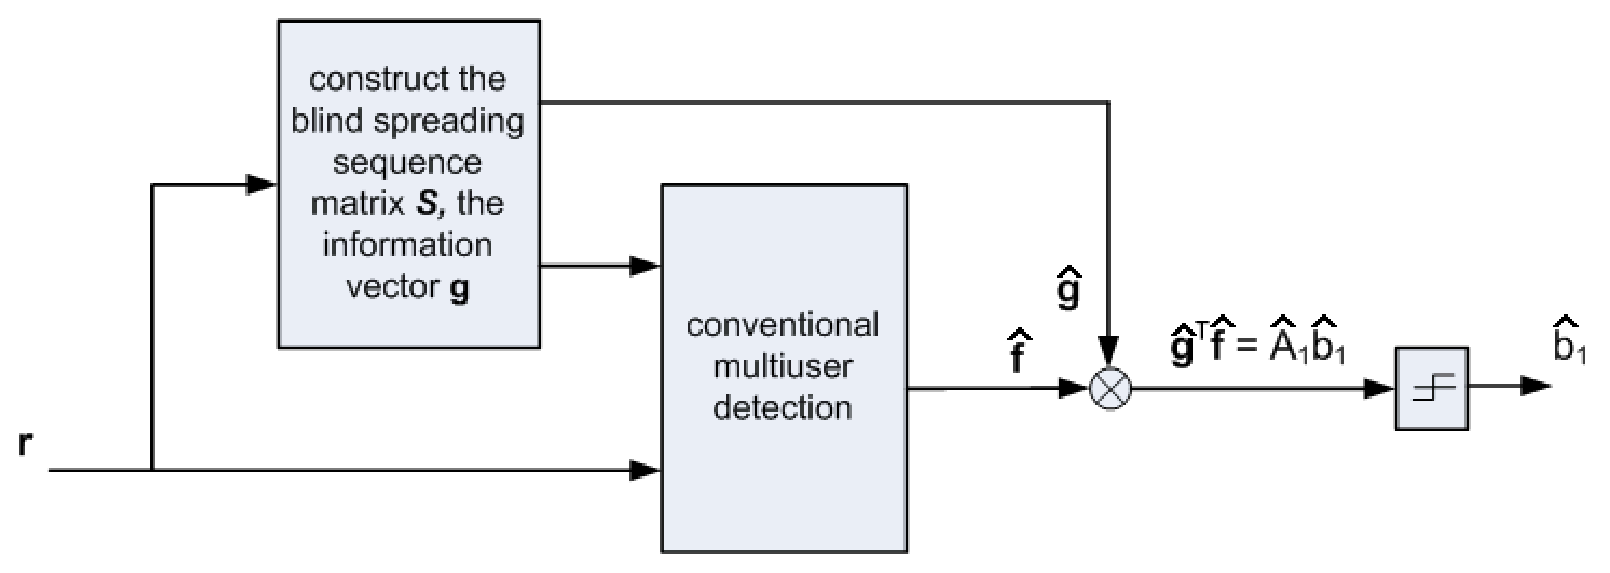
\includegraphics[width=6in]{BMUD_structure1.eps}
\caption{ The proposed blind multiuser detection structure.}
}\label{MUDstruct}
\end{figure}

\subsection{Least-Squares-Based Blind Detections}
Let us start from minimizing least-squared errors. LS-based
algorithms are widely used in practices because they are simple
and easy to be implemented. They only use signal models without
any probabilistic assumptions about data. The negative side, no
claims about optimality can be made and the statistical
performance cannot be assessed without some specific assumption
about the probabilistic structure of the data.

\subsubsection{ Least Squares Detection }
At first, we assume the measurements of $\bcS$ is assumed to be
free of error. All errors are confined to the received vector
$\br$. Hence, the detection vector can be estimated with solving
the following equation

\begin{equation}
\begin{array}{rcl}
{\bbf}_{\rm
LS}=\matrix{\mbox{arg}\min\limits_{\bx}\left\|\br-\bcS\bx\right\|_2}&\mbox{subject
to}&\br\subseteq \mathbb{R}(\bcS)
\end{array}
\label{LSProb}
\end{equation}

Suppose $\bU^T\bcS\bV=\mathbf{\Sigma}$ is the SVD of
$\bcS\in\mathbb{R}^{L\times
 K}$ with $r=\mbox{rank}(\bcS)$. And if $\bU=[\matrix{\bu_1&\bu_2&\ldots&\bu_L}]$,
 $\bV=[\matrix{\bv_1&\bv_2&\ldots&\bv_K}]$, $\mathbf{\Sigma}=\mbox{diag}\{[\matrix{\sigma_1&\ldots\sigma_r&0&\ldots&0}]\}$ and $\br\in \mathbb{R}^{L\times 1}$,
 then LS estimation of $\bbf$ is

 \begin{equation}
 \begin{array}{rcccl}
 \matrix{\bbf_{\rm
 LS}&=&\sum\limits_{i=1}^{r}\frac{\bu_i^T\br}{\sigma_i}\bv_i&=&\bcS^+\br}&=&\bbf + \bcS^+\bar{\bn}
 \end{array}
 \end{equation}

\noindent which minimizes $\|\bcS\bd-\br\|_2$ and has the smallest
2-norm of all minimizers. Moreover
 \begin{equation}
 \matrix{\varepsilon_{\rm LS}^2 &=& \min\limits_{\bx\in\mathbb{R}}\|\bcS\bx-\br\|_2^2 &=& \sum\limits_{i=r+1}^{L}(\bu_i^T\br)^2}
 \end{equation}

\noindent The linear filter representation of the least squares
detector can be written by

\begin{equation}
\begin{array}{rcl}
\bw_{\rm LS}&=&\bcS^{+\rm T}\bg
\end{array}. \label{w_LS}
\end{equation}

\subsubsection{Total Least Squares Estimation }

It assume $\bcS$ to be error-free in the previous LS estimate of
the detection vector $\bbf$. However, this assumption is not
entirely accurate according to the definition of $\bcS$ in
(\ref{S}) since there is a noise term, $\bN$. On the other hand,
$\br$ can also be expressed as
\begin{equation}
\begin{array}{rcl}
\br&=&(\bcS-\bN)\bB^{+}\bb + \bn\\
 &=&\hat{\bcS}\bd + \bn
\end{array}
\end{equation}
where  $\hat{\bcS}=\bcS-\bN=\bS\bB$.  The minimization problem of
(\ref{LSProb}) can then be transformed into the following TLS
problem:
\begin{equation}
\begin{array}{rcl}
\left[\bcS_{\rm TLS},\ \bbf_{\rm
TLS}\right]&=&\matrix{\mbox{arg}\min\limits_{\bar{\bcS},\
\bx}\left\|\left[ \matrix{\bcS&\br} \right] - \left[
\matrix{\bar{\bcS}& \bar{\bcS}\bx}\right]\right\|_2}
\end{array},
\label{TLSProb}
\end{equation}
subject to $\br\subseteq\mathbb{R}(\bar{\bcS})$.

 Let $\bcS=\bU^{'}\mathbf{\Sigma}^{'}\bV^{'T}$ and
$[\bcS\ \br]=\bU\mathbf{\Sigma}\bV^T$ be the SVD of $\bcS$ and
$[\bcS\ \br]$, respectively. If $\sigma_K^{'}
> \sigma_{K+1}$, TLS estimation of $\bbf$ then is
\begin{equation}
\bbf_{\rm TLS} =
\left(\bcS^T\bcS-\sigma_{K+1}^2\bI\right)^{-1}\bcS^T\br
\end{equation}
and
\begin{equation}
\begin{array}{rcl}
\varepsilon_{\rm TLS}^{2}&=&\min\limits_{\bx\in
\mathbb{R}^{K\times
1}}\|\bcS\bx-\br\|_2^2 \\
 &=& \sigma_{K+1}^2\left[1+\sum_{i+1}^{K}\frac{\left(\bu_i^{'T}\br\right)^2}
{\sigma_i^{'2}-\sigma_{K+1}^2}\right]
\end{array}
\end{equation}
where $\bU=[\bu_1\ \bu_2\ \ldots\ \bu_L]$, $\bV=[\bv_1\ \bv_2\
\ldots\ \bv_{K+1}]$, $\mathbf{\Sigma}={\rm diag}\{[\sigma_1\
\sigma_2 \ldots\ \sigma_{K+\min\limits\{L-K,\ 1\}}]\}$ and
$\bU^{'}=[\bu_1^{'}\ \bu_2^{'}\ \ldots\ \bu_L^{'}]$,
 $\bV^{'}=[\bv_1^{'}\ \bv_2^{'}\ \ldots\ \bv_{K}^{'}]$,
 $\mathbf{\Sigma}^{'}={\rm diag}\{[\sigma_1^{'}\ \sigma_2^{'}\ \ldots\
 \sigma_K^{'}]\}$. And the linear filter $\bw_{\rm TLS}$ is

\begin{equation}
\begin{array}{rcl}
\bw_{\rm TLS}&=&\bcS(\bcS^{\rm T}\bcS-\sigma_{K+1}^2\bI)^{-1}\bg
\end{array}
\end{equation}

\subsubsection{Mixed LS/TLS Detection}

In the LS problem of (\ref{LSProb}), it assumed the blind
signature matrix $\bcS$ is error-free. Again, this assumption is
not completely accurate. In the TLS problem of (\ref{TLSProb}), it
assumed that in each column of the blind signature matrix, $\bcS$,
some noise or error exists.  This assumption also is not complete.
Though there exists a noise or error matrix $\bN$ in $\bcS$ from
(\ref{S}), its first column is exactly known to be noise-free or
error-free.  Hence, to maximize the estimation accuracy of the
detection vector $\bbf$, it is natural to require that the
corresponding columns of $\bcS$ be unperturbed since they are
known exactly. The problem  of estimating the detection vector
$\bd$ can then be transformed into the following MLS problem by
considering (\ref{LSProb}) and (\ref{TLSProb}):
\begin{equation}
\begin{array}{rcl}
\left[\bcS_{\rm MLS},\ \bbf_{\rm MLS}\right] &=
&\matrix{\mbox{arg}\min\limits_{\bar{\bcS},\
\bx}\left\|\left[\matrix{\tilde{\bcS}&\br}\right]-\left[\matrix{\bar{\bcS}&[\bs_1\
 \bar{\bcS}]\bx}\right]\right\|_{2} }
\end{array}\label{MLSProb}
\end{equation}
subject to $\br\subseteq\mathbb{R}\left([\bs_1\
\bar{\bcS}]\right)$. The following lemma outlines the MLS
solution.

Consider the MLS problem in (\ref{MLSProb}) and perform the
Householder transformation $\bQ$ on the matrix
$[\matrix{\bcS&\br}]$ so that
\begin{equation}
\begin{array}{rcl}
\bQ^{\rm
T}[\matrix{\bs_1&\bar{\bcS}&\br}]&=&\left[\matrix{R_{11}&\bR_{12}&R_{1r}\cr
\mathbf{0}&\bR_{22}&\bR_{2r}}\right]
\end{array}
\end{equation}
where $R_{11}= A_1$, $\bR_{12}$ is a $1\times (M-1)$ vector,
$\bR_{22}$ is a $(L-1)\times (M-1)$ matrix and $\bR_{2r}$ is a
$(L-1)\times 1$ vector and

\begin{equation}
\begin{array}{rcl}
\bQ &=&\bI - \frac{1}{A_1(A_1-s_{11})}\left[\matrix{s_{11}-A_1\cr
s_{12}\cr \vdots \cr s_{1L}}\right]\left[\matrix{(s_{11}-A_1)&
s_{12}& \cdots & s_{1L}}\right]
\end{array}
\end{equation}



Denote $\sigma'$ as the smallest singular value of $\bR_{22}$ and
$\sigma$ as the smallest singular value of
$[\matrix{\bR_{22}&\bR_{2r}}]$. If $\sigma'>\sigma$, then the MLS
solution uniquely exists and is given by
\begin{equation}
\begin{array}{rcl}
\bbf_{\rm
MLS}&=&\left(\bcS^T\bcS-\sigma^2\left[\matrix{0&\mathbf{0}\cr\mathbf{0}&\mathbf{I}_{M-1}}\right]\right)^{-1}\bcS^T\br
\end{array}.
\end{equation}

\noindent The linear filter representation of this MLS detection
is

\begin{equation}
\begin{array}{rcl}
\bw_{\rm
MLS}&=&\bcS\left(\bcS^T\bcS-\sigma^2\left[\matrix{0&\mathbf{0}\cr\mathbf{0}&\mathbf{I}_{M-1}}\right]\right)^{-1}\bg
\end{array}.
\end{equation}




\subsection{Best Linear Unbiased Detection}

We begin by assuming the linear structure

\begin{equation}
\begin{array}{rcl}
{\bbf}_{\rm BLU}&=&\bW_{\rm BLU}^{\rm T}\br
\end{array}
\end{equation}

\noindent for this so-called best linear unbiased estimator
(BLUE). Matrix $\bW_{\rm BLU}$ is designed such that: 1) $\bcS$
must be deterministic, and 2) $\bar{\bn}$ must be zero mean with
positive definite known covariance matrix $\bC_{\bar{\bn}}$, 3)
${\bbf}_{\rm BLU}$ is an unbiased estimator of $\bbf$, and 4) the
error variance for each of the $M$ parameters is minimized as

\begin{equation}
\begin{array}{rcl}
\bW_{\rm BLU}&=&\min\limits_{\bW_{\bbf}}
\mbox{var}\left\{\bW_{\bbf}^{\rm T}\br\right\}
\end{array}
\end{equation}

In this way, ${\bbf}_{\rm BLU}$ will be unbiased and efficient,
within the class of linear estimators, by design. The resulting
best linear unbiased estimator is (Gauss-Markov Theorem):

\begin{equation}
\begin{array}{rcl}
{\bW}_{\rm BLU}&=&\bC_{\bar{\bn}}^{-1}\bcS(\bcS^{\rm
T}\bC_{\bar{\bn}}^{-1}\bcS)^{-1}
\end{array}
\end{equation}

\noindent and

\begin{equation}
\begin{array}{rcl}
{\bbf}_{\rm BLU}&=&\bW_{\rm BLU}^{\rm T}\br\\
 &=&(\bcS^{\rm
T}\bC_{\bar{\bn}}^{-1}\bcS)^{-1}\bcS^{\rm
T}\bC_{\bar{\bn}}^{-1}\br\ .
\end{array} \label{BLUE}
\end{equation}

\noindent The covariance matrix of ${\bbf}_{\rm BLU}$ given by

\begin{equation}
\begin{array}{rcl}
{\bC}_{\bbf_{\rm BLU}}&=&(\bcS^{\rm
T}\bC_{\bar{\bn}}^{-1}\bcS)^{-1}
\end{array}.
\end{equation}

\noindent Since the above data are of Gaussian distributions, the
BLUE in (\ref{BLUE}) is also the minimum variance unbiased
estimation. The linear filter representation of this detector is

\begin{equation}
\begin{array}{rcl}
{\bw}_{\rm BLU}$=$\bC_{\bar{\bn}}^{-T}\bcS(\bcS^{\rm
T}\bC_{\bar{\bn}}^{-1}\bcS)^{-1}\bg
\end{array}.\label{w_BLUE}
\end{equation}

Now the question is how we know about $\bC_{\bar{\bn}}^{-1}$. With
(\ref{var_n}), $\bC_{\bar{\bn}}^{-1}$ can be decided by $\sigma^2$
and $\bC_{\bbf}$. Let us consider $\bC_{\bbf}$ first.




Though the PDF of $\bB$ may be determined, the PDF of $\bB^{+}$ is
largely unknown. This makes it is hard to calculate the
closed-form solution of $\bC_{\bbf}$ and $\bC_{\tilde{\bn}}$.
However, with Girko's Law, when $\alpha=(K-1)/(M-1)$ is fixed,
$K$, $M$ $\rightarrow\infty$, the diagonal element of
$\frac{1}{M-1}\tilde{\bD}^+\tilde{\bb}\tilde{\bb}^{\rm
T}\tilde{\bD}^{\rm +T}$ may be approximated
by~\cite{Muller,Hanly90}

\begin{equation}
\begin{array}{rcl}
\frac{1}{M-1}\left[\tilde{\bD}^+\tilde{\bb}\tilde{\bb}^{\rm
T}\tilde{\bD}^{\rm +T}\right]_{ii}^{-1}&\rightarrow&1-\alpha
\end{array}.
\end{equation}

\noindent So, $\bC_{\bbf}$ can be approximated by

\begin{equation}
\begin{array}{rcl}
\bC_{\bbf}&=&\mbox{E}\left\{\bbf\bbf^{\rm T}\right\}\\
&=&\mbox{E}\left\{\left[\matrix{(A_1b_1-\bd^{\rm
T}\tilde{\bD}^{\rm +}\tilde{\bb})^2&(A_1b_1-\bd^{\rm
T}\tilde{\bD}^{\rm +}\tilde{\bb})\tilde{\bb}^{\rm
T}\tilde{\bD}^{\rm +T}\cr (A_1b_1-\bd^{\rm T}\tilde{\bD}^{\rm
+}\tilde{\bb})\tilde{\bD}^+\tilde{\bb}&
\tilde{\bD}^+\tilde{\bb}\tilde{\bb}^{\rm T}\tilde{\bD}^{\rm
+T}}\right]\right\}\\
&\approx&\left[\matrix{\frac{2M-K-1}{M-K}A_1^2&\bzero^{\rm
T}\cr\bzero&\frac{1}{M-K}\bI}\right]
\end{array}
\end{equation}


Now, the following result could be easily obtained.


\subsection{Linear Minimum Mean Squared Detection}
Now we propose a linear estimator based on MMSE criterion. This
class of estimators are generically termed Wiener filter. Given
measurements $\br$, the MSE estimator of $\bbf$, ${\bbf}_{\rm MS}
= f( \br )$, minimizes the mean-squared error $J_{\rm
MS}=E\{||\bbf-\hat{\bbf}||_2^2\}$. The function $f(\br)$ may be
nonlinear or linear and its exact structure is determined by
minimizing $J_{\rm MS}$. When $\bbf$ and $\br$ are jointly
Gaussian, the linear estimator $\bW_{\rm MS}$ that minimizes the
mean-sqared error is (Bayesian Gauss-Markov Theorem)

\begin{equation}
\begin{array}{rcl}
{\bW}_{\rm MS} &=&
\bC_{\bar{\bn}}^{-1}\bcS(\bC_{\bbf}^{-1}+\bcS^{\rm
T}\bC_{\bar{\bn}}^{-1}\bcS)^{-1}
\end{array}\label{W_MSE}
\end{equation}

\noindent and

\begin{equation}
\begin{array}{rcccl}
{\bbf}_{\rm MS} &=&{\bW}_{\rm MS}^{\rm T}\br
&=&(\bC_{\bbf}^{-1}+\bcS^{\rm
T}\bC_{\bar{\bn}}^{-1}\bcS)^{-1}\bcS^{\rm
T}\bC_{\bar{\bn}}^{-1}\br
\end{array}. \label{MSE}
\end{equation}

\noindent The performance of the linear MMSE estimator is measured
by the error vector $\mathbf{\varepsilon_{\rm MS}}=\bbf-\bbf_{\rm
MS}$ whose mean is zero and covariance matrix is

\begin{equation}
\begin{array}{rcl}
\bC_{\mathbf{\varepsilon_{\rm MS}}} &=& (\bC_{\bbf}^{-1}+\bcS^{\rm
T}\bC_{\bar{\bn}}^{-1}\bcS)^{-1}
\end{array}.
\end{equation}

The linear filter representation of the blind linear MMSE detector
with $\bbf_{\rm MS}$ is

\begin{equation}
\begin{array}{rcl}
{\bw}_{\rm MS}&=&
\bC_{\bar{\bn}}^{-T}\bcS(\bC_{\bbf}^{-1}+\bcS^{\rm
T}\bC_{\bar{\bn}}^{-1}\bcS)^{-1}\bg
\end{array} \label{w_MSE}
\end{equation}

\pagebreak

\section{ Considerations On Adaptive Updating}

\begin{figure}
\center{
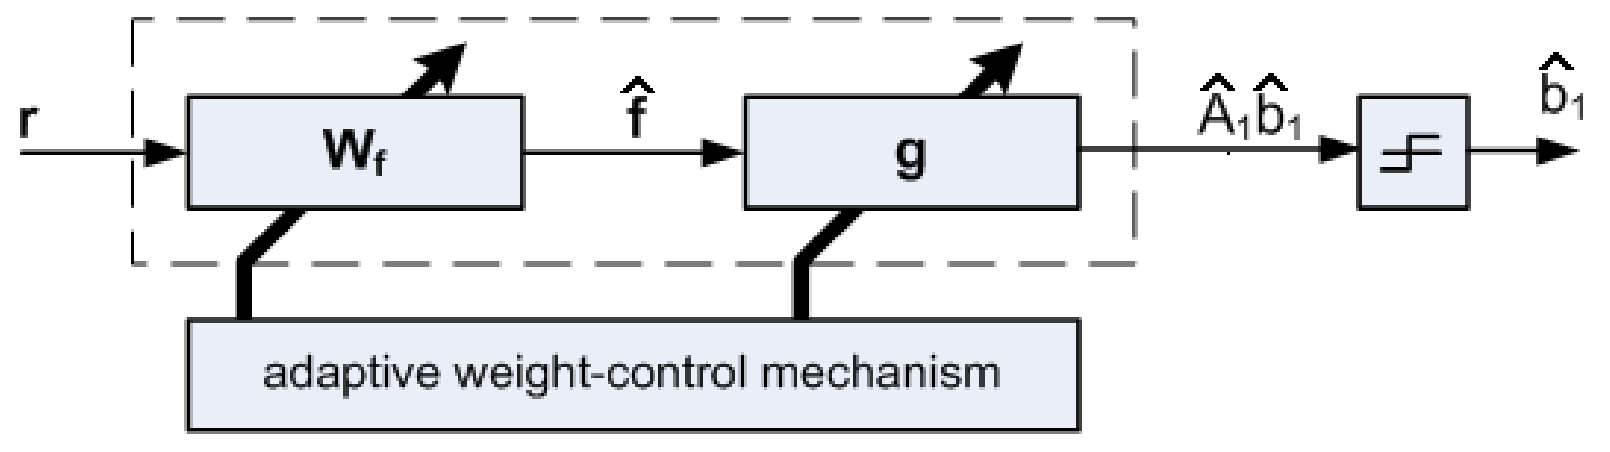
\includegraphics[width=6in]{BMUD_structure5.eps}
\caption{ The proposed adaptive blind multiuser detection
structure.} }\label{AMUDstruct}
\end{figure}

\subsection{Least Mean Square Detection}

The optimum tap-weights of a transversal (FIR) Wiener filter can
be obtained by solving the Wiener-Hopf equation provided that the
required statistics of the underlying signals are available. An
alternative way of finding the optimum tap-weights is to use an
iterative search algorithm that starts at some arbitrary initial
point in the tap-weight vector space and progressively moves
towards the optimum point in steps. There are many iterative
search algorithms derived for minimizing the underlying cost
function with the true statistics replaced by their estimate
obtained in some manner.



\subsection{Kalman Filtering Detection} Kalman filter can be
taken as an important generalization of Wiener filter with the
ability to accommodate vector signals and noise which additionally
may be nonstationary. It may also be thought of as a sequential
MMSE estimator of a signal embedded in noise and this signal can
be characterized by a state model. If the signal and noise are
jointly Gaussian, then the Kalman filter is an optimal MMSE
estimator, and if not, it is the optimal linear MMSE estimator. To
develop a blind adaptive multiuser detector based on Kalman
filtering in~(\ref{KFE_SF_X}) and (\ref{KFE_SF_Y}), a linear
first-order state space model have to be devised.


\begin{equation}
\begin{array}{rcl}
\mathbf{x}[n]&=&\mathbf{P}\mathbf{x}[n-1] +
\mathbf{Q}\mathbf{u}[n]
\end{array} \label{KFE_SF_X}
\end{equation}

\begin{equation}
\begin{array}{rcl}
\mathbf{y}[n]&=&\mathbf{H}\mathbf{x}[n] + \mathbf{w}[n]
\end{array} \label{KFE_SF_Y}
\end{equation}


\pagebreak

\bibliographystyle{unsrt}
\bibliography{FastBDD}

\end{document}
